\subsection{Overview}
We chose the three tier architecture for S\&C because we believe that it is a solid choice aligned with our goals and requirements.
The architecture is divided in three:
\begin{enumerate}
    \item\textbf{Presentation Tier}:
    This is essentially the user interface
    \item\textbf{Application Tier}:
    This layer is where the data are transformed and undergo a set of processes to make them available to the user interface
    \item\textbf{Data Tier}:
    This layer is where the data are stored and managed remotely.
\end{enumerate}
This is the visualization of the 3-tier logic. \cite{3Tier}\\
\begin{figure}[h!]
        \centering  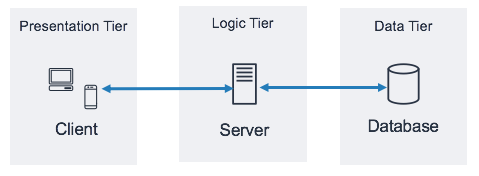
\includegraphics[width=1\textwidth]{DD/Images/aws.png}
        \label{fig:3Tier}
\end{figure}
\\
We also chose to use REST APIs to make the presentation layer and application layer communicate.  \\
The following image displays how an API works\cite{REST}:
\begin{figure}[h!]
        \centering  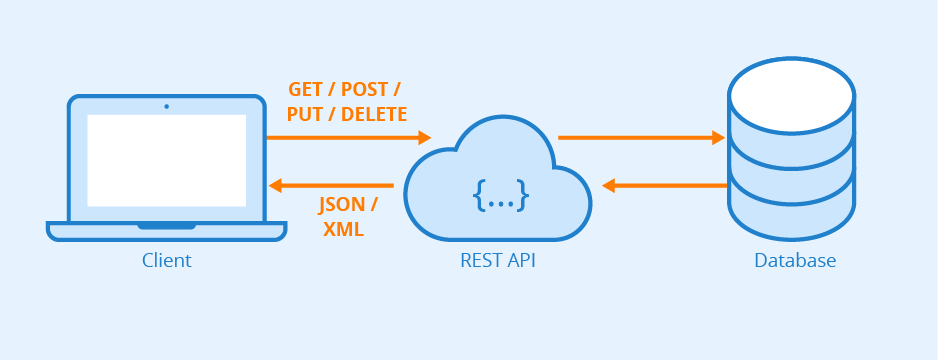
\includegraphics[width=1\textwidth]{DD/Images/rest.png}
        \label{fig:RESTAPI}
\end{figure}
\newpage
\subsection{Component View}
This section aims to give a general representation of the core components of the system and how they interact together without focusing on the internal details.
Indeed it is important to grasp the division in modules and the interactions among them. In the component view image it is clearly distinguishable the 3-tier architecture and composed by the WebApp, the Back-End composed by all the modules depicted and listed below and the Database. Since all the logic is implemented in the middle layer, namely the S\&C Server, that is where all the modules are and interact.
The main components of the back-end are:
\begin{enumerate}
    \item \textbf{WebApp}: it is the component in charge of providing the user interface for interacting with the system. It relies on the API to fetch and send data for various operations.
    \item \textbf{S\&C Server}
    \begin{itemize}
        \item \textbf{SearchManager}: it is the component in charge of receiving and handling the search requests about the internship positions issued by the students 
        \item \textbf{RegistrationManager}: it is the component in charge of managing the registration of the users.
        \item \textbf{LoginManager}: it is the component in charge of the login of the users
        \item \textbf{NotificationManager}: it is the component in charge of sending the notifications to users, including push notifications and confirmation emails used to validate email accounts in the registration process
        \item \textbf{ProfileManager}: it is the component in charge of handling user profile information. It is supposed dot interact with all the other components in order to keep the profile of the user up to date.
        \item \textbf{InternshipManager}: it is the component in charge of managing the internships. It manages the internship status, the communication, the assessment process (if needed), publishing of news related to the internships.
        \item \textbf{ApplicationManager}: it is the component in charge of keeping track of the status application and its details.
        \item \textbf{API}: it is the component that allows the back-end to interact with the requests from the front-end.
    \end{itemize}
    \item \textbf{Database}: it is the component in charge of storing all the information relevant to the platform.


\end{enumerate}
\newpage
\begin{figure}[h!]
        \centering  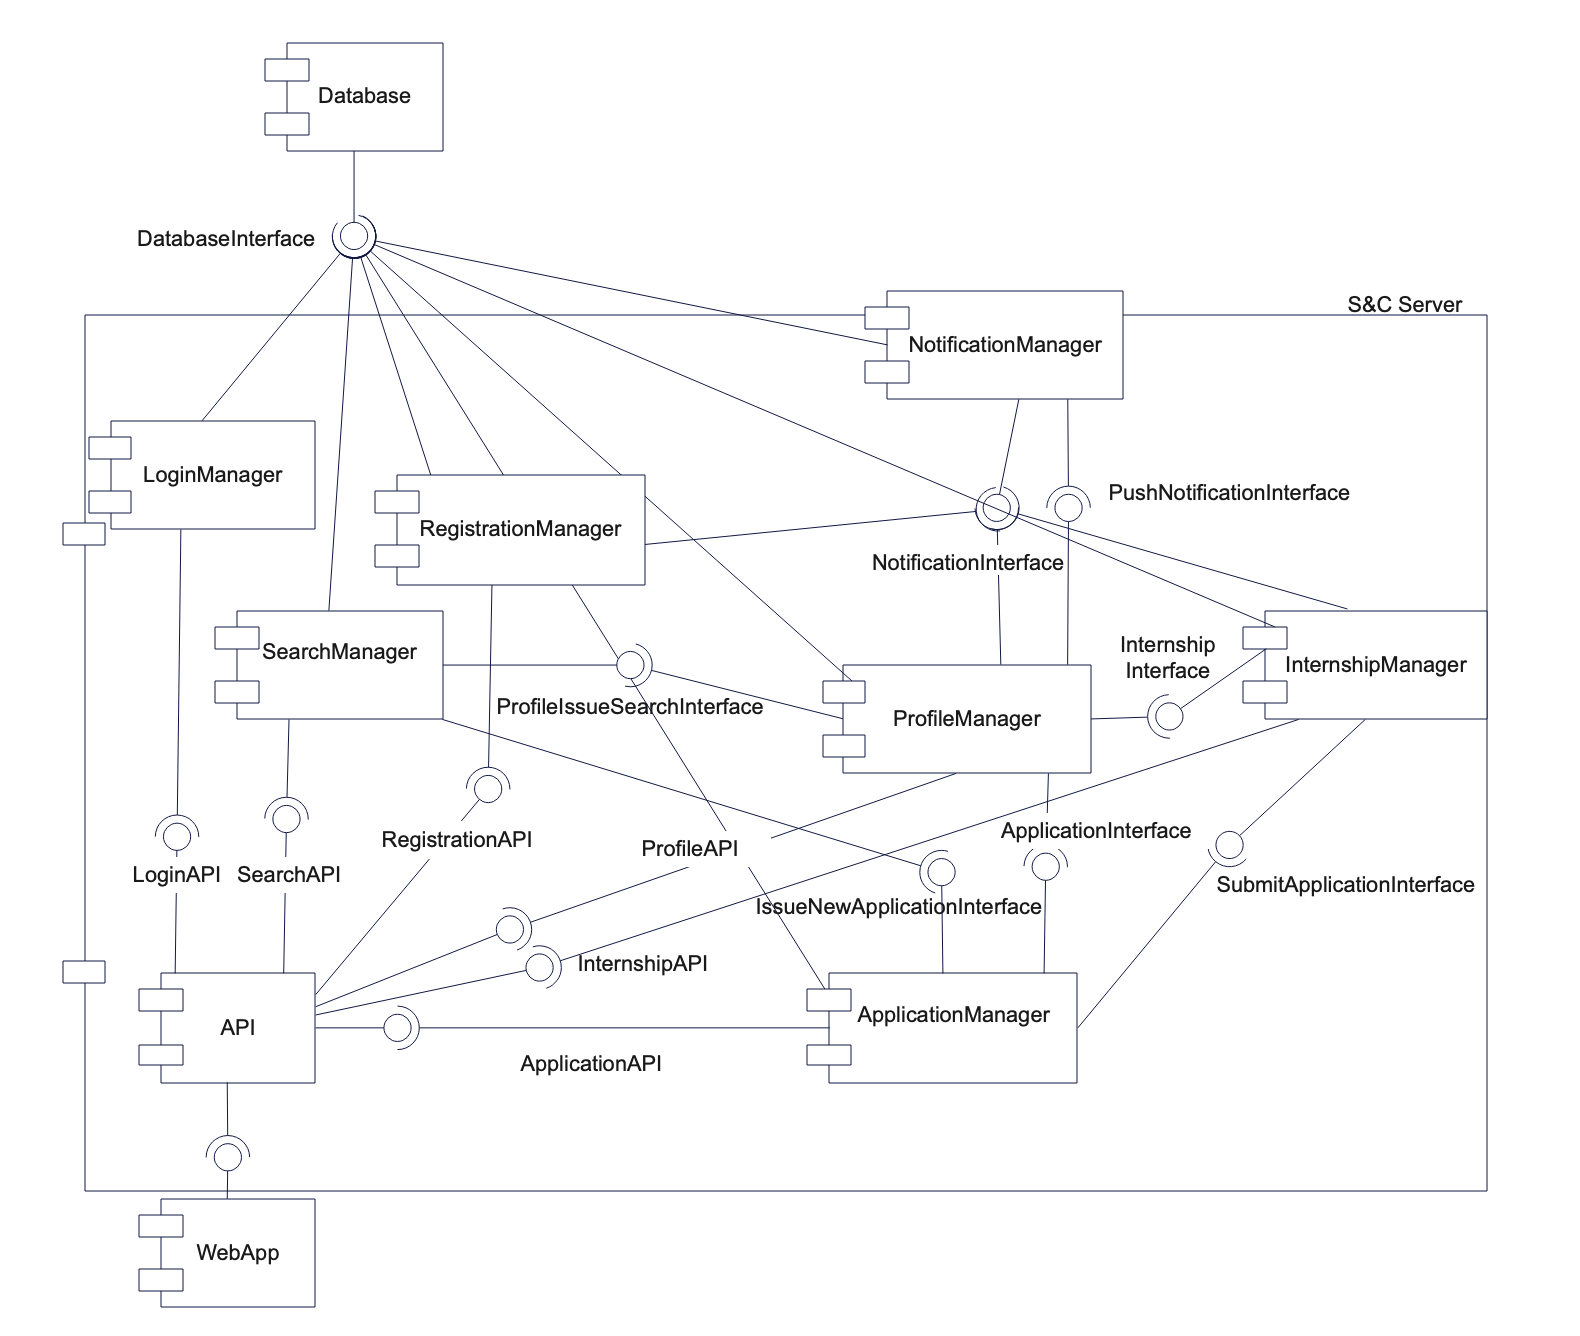
\includegraphics[width=1\textwidth]{DD/Images/CD.png}
        \label{fig:ComponentViewDiagram}
\end{figure}
\newpage

\newpage
\subsection{Runtime View}

\begin{enumerate}
    % -- INT01 --
    \item \textbf{User Login}
    \begin{figure}[h!]
            \centering  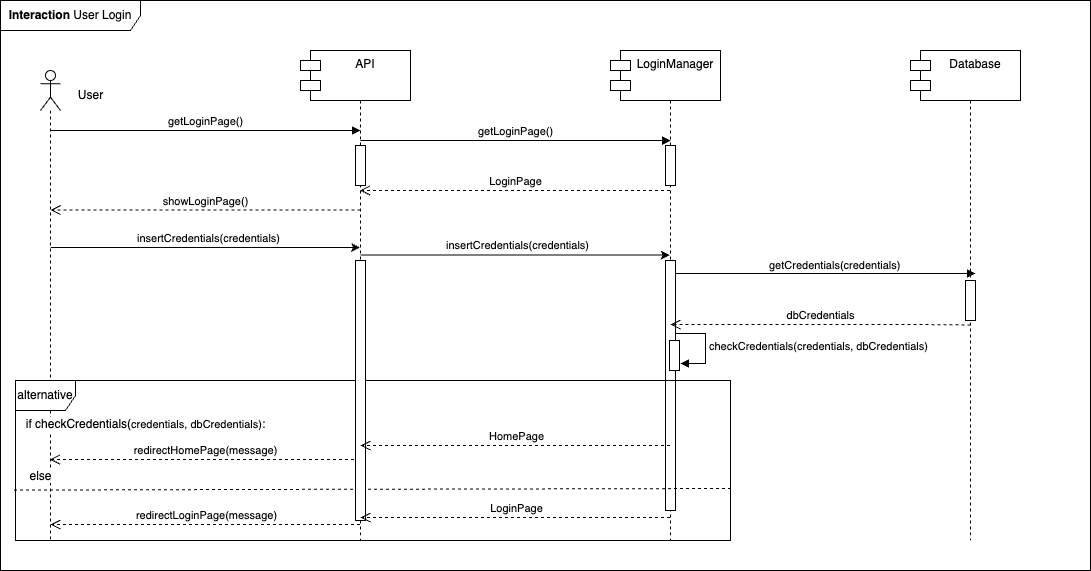
\includegraphics[width=1\textwidth]{DD/Images/Interactions/INT01_UserLogin.drawio.png}
            \label{fig:ComponentViewDiagram}
            \caption*{The interaction diagram shows the process of a user logging into S\&C. The sequence begins with the user requesting the login page through the API. The API retrieves and displays the login page for the user to interact with. Once the user inputs their credentials, such as a username and password, these are submitted to the API. The API then forwards the credentials to the LoginManager, which is responsible for handling the authentication process. The LoginManager communicates with the Database to retrieve the stored credentials associated with the submitted user details. After getting the stored credentials, the LoginManager compares them with the provided ones to check the user's identity. If the credentials match, the validation is successful and the user is redirected to the homepage. If the credentials do not match, an error is raised and the user is redirected to the login page.
            }
    \end{figure}


% -- INT02 --
    \newpage
    \item \textbf{User Logout}
    \begin{figure}[h!]
            \centering  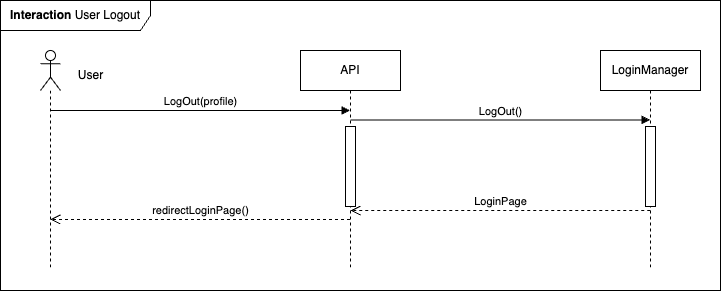
\includegraphics[width=1\textwidth]{DD/Images/Interactions/INT02_UserLogout.drawio.png}
            \label{fig:ComponentViewDiagram}
            \caption*{The interaction diagram describes the process of a user logging out from S\&C The sequence begins with the user starting the logout operation by sending a request to the API, specifying their profile. The API forwards this request to the LoginManager, which is responsible for handling session management and user authentication. The LoginManager then closes the user's session and clears any associated session data. Once the session is successfully invalidated, the LoginManager informs the API that the user has been logged out. The API then redirects the user to the login page, notifies the completion of the logout process.
            }
    \end{figure}

    % -- INT03 --
    \newpage
    \item \textbf{User Update}
    \begin{figure}[h!]
            \centering  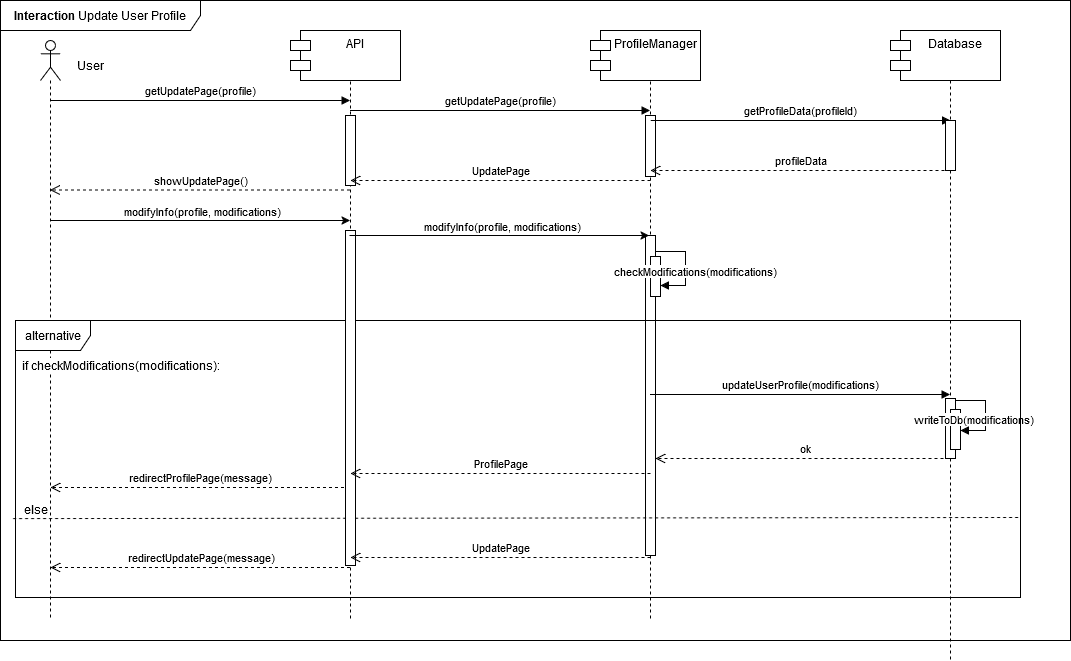
\includegraphics[width=1\textwidth]{DD/Images/Interactions/INT03_UserUpdate.drawio.png}
            \label{fig:ComponentViewDiagram}
            \caption*{The interaction diagram shows the process of updating a user profile in S\&C. The sequence begins with the user requesting the profile update page by sending their profile information to the API. The API forwards this request to the ProfileManager, which retrieves the data that can be updated  from the Database. The API then displays the update page with the pre-compiled data to the user.
            Once the user makes changes to their profile and submits the modifications, the API sends the updated information to the ProfileManager for processing. The ProfileManager validates the submitted modifications through its internal logic. If the modifications are valid, the ProfileManager writes the changes to the Database.
            the user is redirected to their profile page. If the update fails due to an error, the API redirects the user back to the update page with an error message.}
    \end{figure}

    % -- INT04 --
    \newpage
    \item \textbf{Student Registration}
    \begin{figure}[h!]
            \centering  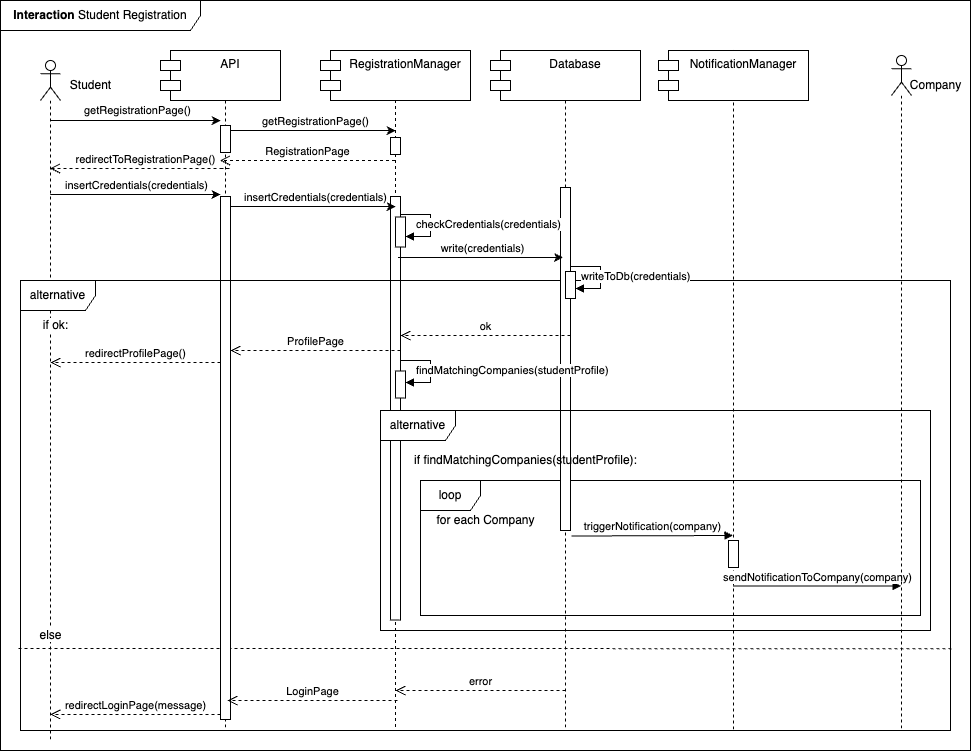
\includegraphics[width=1\textwidth]{DD/Images/Interactions/INT04_StudentRegistration.drawio.png}
            \label{fig:ComponentViewDiagram}
            \caption*{The interaction diagram shows the process of a student registering within S\&C. The process begins when the student requests access to the registration page through the API. The API retrieves the registration interface by interacting with the RegistrationManager, which provides the appropriate page. The API then displays the registration page to the student. Once the student submits their credentials, the API forwards the submitted data to the RegistrationManager, which validates the credentials to ensure they meet the required standards. If the credentials are valid, the RegistrationManager saves the student’s data to the Database. Upon successful storage, the RegistrationManager proceeds to find matching companies based on the student’s profile. If relevant companies are identified, the RegistrationManager triggers the NotificationManager to send notifications to these companies, informing them of the newly available student profile. If the credentials are evaluated correct, the API redirects the student to their profile page. Otherwise the RegistrationManager communicates the problem to the API, which redirects the student back to the login page displaying an error message.
            }
    \end{figure}

    % -- INT05 --
    \newpage
    \item \textbf{Internship Search}
    \begin{figure}[h!]
            \centering  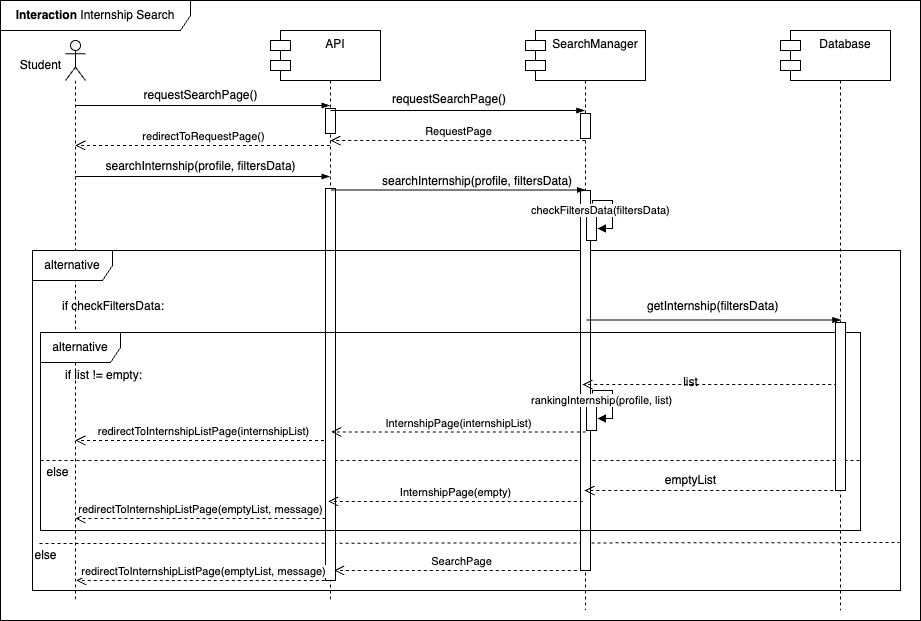
\includegraphics[width=1\textwidth]{DD/Images/Interactions/INT05_InternshipSearch.drawio.png}
            \label{fig:ComponentViewDiagram}
            \caption*{The interaction diagram describes the process of searching for internship positions within S\&C. The sequence begins when the user requests access to the internship search page through the API. The API processes this request and redirects the user to the internship search page. Once on the search page, the user provides search criteria, which may include filters values but also keywords. These data are sent from the API to the SearchManager to be validated and if they are evaluated correct, the SearchManager uses them to query the Database for matching internships. If the Database returns a list of internships that match the user's criteria, the SearchManager runs a ranking algorithm on them to put first the most suited ones to the profile who issued the search, then the API redirects the user to the internship results page and displays the available options. If no matches are found, the API redirects the user to an empty internship results page, along with a message indicating that no internship meets the specified criteria. 
            }
    \end{figure}

    % -- INT06 --
    \newpage
    \item \textbf{Internship Application}
    \begin{figure}[h!]
            \centering  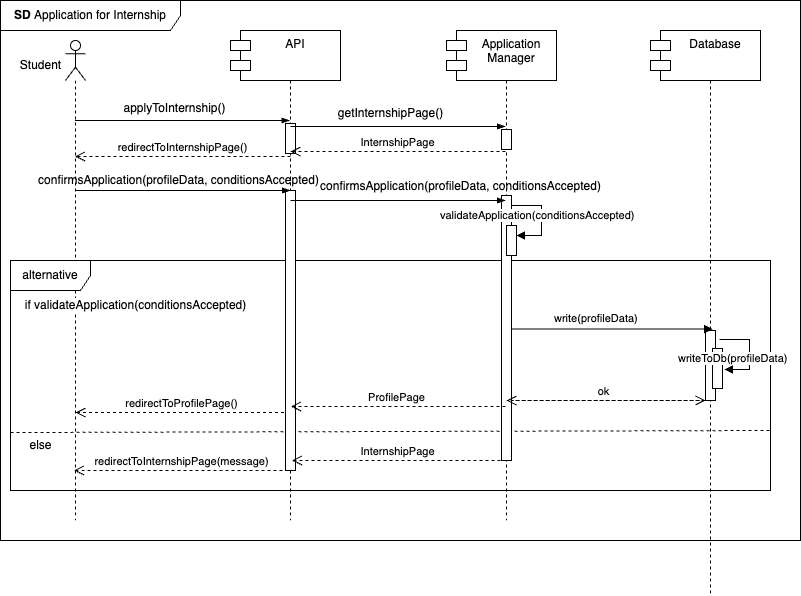
\includegraphics[width=1\textwidth]{DD/Images/Interactions/INT06_InternshipApplication.drawio.png}
            \label{fig:ComponentViewDiagram}
            \caption*{
            The interaction diagram shows the process of applying for an internship within S\&C. The sequence begins when the user accesses the internship application page by interacting with the API. The API redirects the user to the internship position page where he/she must accept the terms and conditions. Once the user submits their application, the API forwards the data to the Application Manager, which validates the submission. This validation includes ensuring that the user has accepted the terms and conditions of the internship application. If the validation is successful, the Application Manager writes the relevant profile data to the Database to store the application and then the API redirects the user to their profile page to confirm the completion of the application process.
            If the validation fails the API keeps the user into the internship application page showing an error message.
            }
    \end{figure}

    % -- INT07 --
    \newpage
    \item \textbf{Student Examines Application}
    \begin{figure}[h!]
            \centering  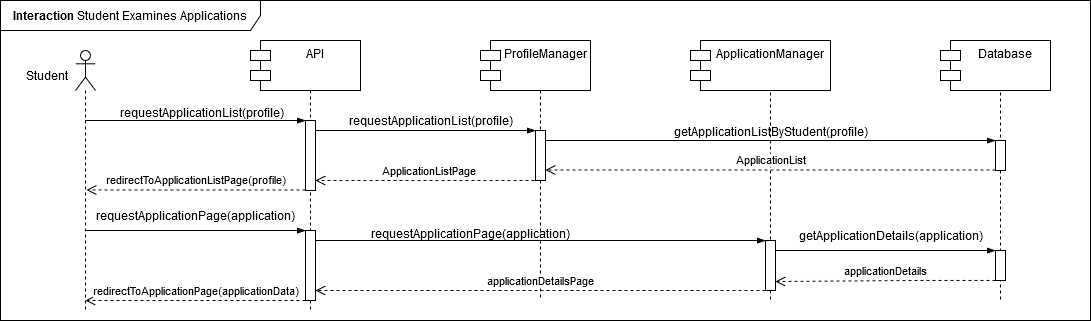
\includegraphics[width=1\textwidth]{DD/Images/Interactions/INT07_StudentExaminesApplications.drawio.png}
            \label{fig:ComponentViewDiagram}
            \caption*{The interaction diagram shows the process of a student examining their internship applications within S\&C. The process begins when the user requests to view their application history. This request is handled by the API, which redirects the user to the application list page. The API communicates with the ProfileManager to retrieve the user’s profile-related data and then queries the ApplicationManager for a list of the student’s applications.
            The ApplicationManager consults the Database to gather the details of all internship applications associated with the user. Once the information is retrieved, it is sent back to the API, which displays the application list to the user on the application list page.
            If the user selects a specific application to examine in more detail, the API processes this request by communicating with the ApplicationManager. The ApplicationManager retrieves the details of the selected application from the Database and sends them back to the API. Finally, the API redirects the user to a detailed view of the selected application, where they can review the information related to it.
            }
    \end{figure}

    % -- INT08 --
    \newpage
    \item \textbf{Company Registration}
    \begin{figure}[h!]
            \centering  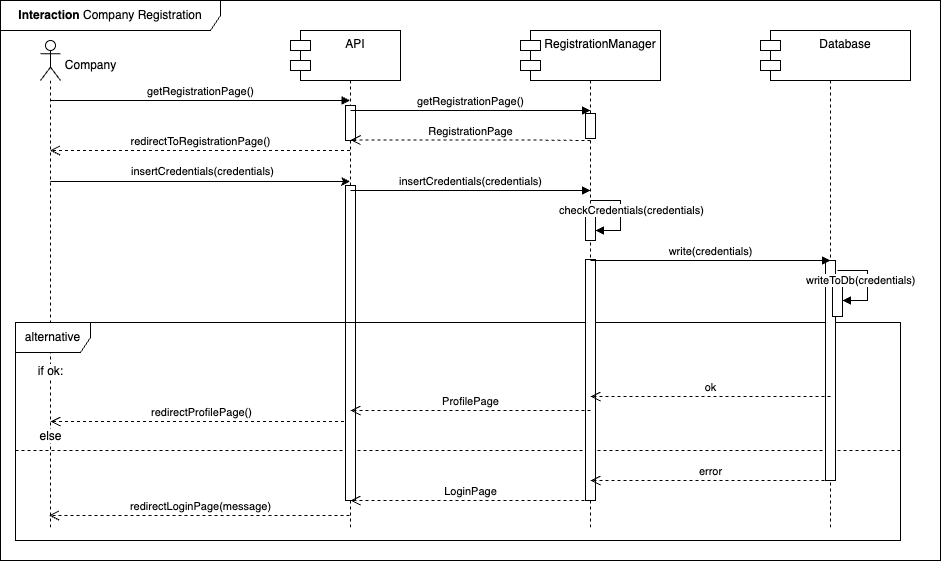
\includegraphics[width=1\textwidth]{DD/Images/Interactions/INT08_CompanyRegistration.drawio.png}
            \label{fig:ComponentViewDiagram}
            \caption*{The interaction diagram describes the process of company registration within the S\&C. The process begins when a company starting a request to access the registration page. The API handles this request and redirects the company to the appropriate page for inputting registration details. Once the company provides its credentials, the API forwards the submitted information to the RegistrationManager that validates them, checking their correctness and ensuring they meet the necessary requirements. If the validation is successful, the RegistrationManager stores the new credentials by writing them to the Database. After confirmation of successful storage, the API redirects the company to their newly created profile page. If the credentials fail validation due to errors or missing information, the RegistrationManager notifies the API. In this case, the API redirects the company back to the login page with an appropriate error message.
            }
    \end{figure}

    % -- INT09 --
    \newpage
    \item \textbf{Post a new Internship}
    \begin{figure}[h!]
            \centering  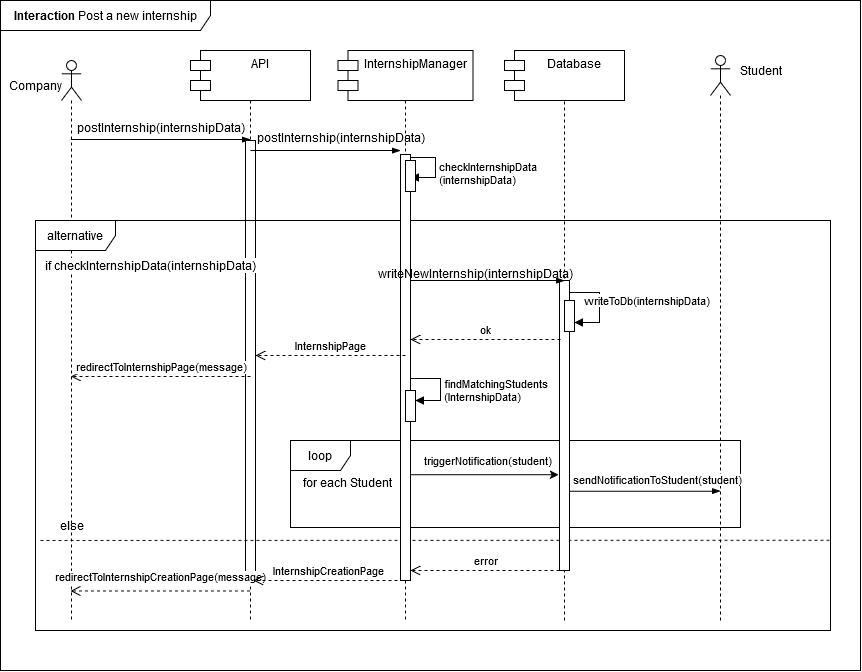
\includegraphics[width=1\textwidth]{DD/Images/Interactions/INT09_PostNewInternship.drawio.png}
            \label{fig:ComponentViewDiagram}
            \caption*{The interaction diagram describes the process of posting a new internship position within S\&C. The sequence starts with a company accessing the internship creation page through the API. On this page, the user inputs all the relevant details for the internship position, which the API forwards to the InternshipManager. The InternshipManager is responsible for validating the provided internship data to ensure it meets the required standards and format. If the data passes validation, the InternshipManager stores the internship information in the Database. After successfully saving the data, the InternshipManager proceeds to identify students whose profiles match the specified internship criteria. For each matched student, a notification is triggered by the InternshipManager and sent to the student, informing them of the new internship opportunity. In cases where the validation process fails due to incomplete or incorrect data, the InternshipManager informs the API of the issue. The API then redirects the user back to the internship creation page, providing a message with details about the error.
            }       
    \end{figure}

    % -- INT10 --
    \newpage
    \item \textbf{Close an Internship}
    \begin{figure}[h!]
            \centering  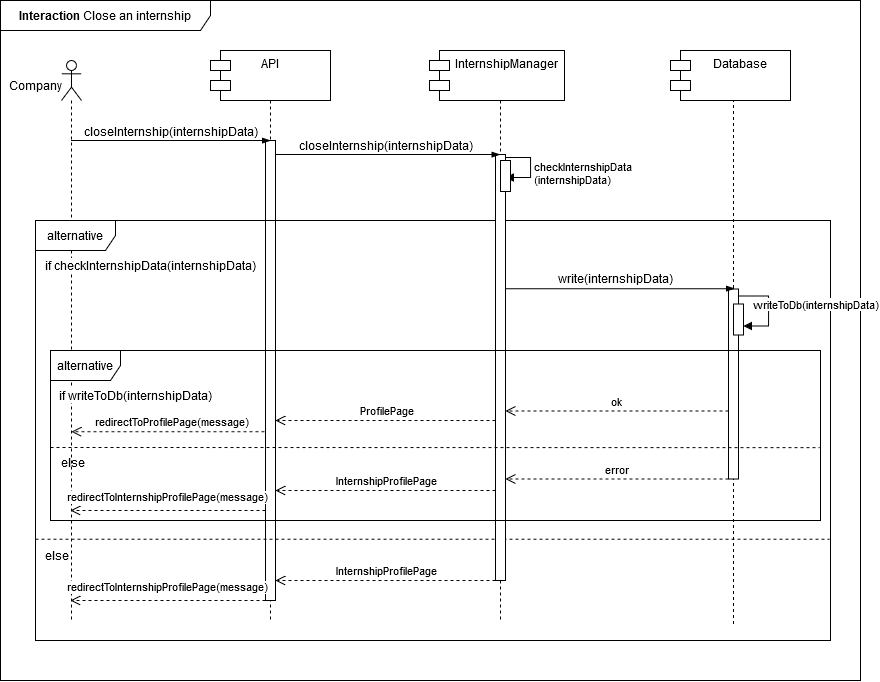
\includegraphics[width=1\textwidth]{DD/Images/Interactions/INT10_CloseInternship.drawio.png}
            \label{fig:ComponentViewDiagram}
            \caption*{The interaction diagram describes the process of closing an internship position within S\&C. The sequence starts with a company pressing "Close" button that inform the \textbf{InternshipManager} through the \textbf{API} the desire to close a specific internship. 
            The \textbf{InternshipManager} is responsible for validating the provided internship data to ensure it meets the required standards, format and the membership of the internship to the specific company. If the data passes validation, the \textbf{InternshipManager} changes the internship information in the \textbf{Database}. In cases where the validation process fails due to incomplete or incorrect data, the \textbf{InternshipManager} informs the \textbf{API} of the issue. The \textbf{API} then redirects the user back to the internship profile page, providing a message with details about the error, otherwise the company is redirected to its profile page.
            }         
    \end{figure}

    % -- INT11 --
    \newpage
    \item \textbf{Company Examines Internship Positions}
    \begin{figure}[h!]
            \centering  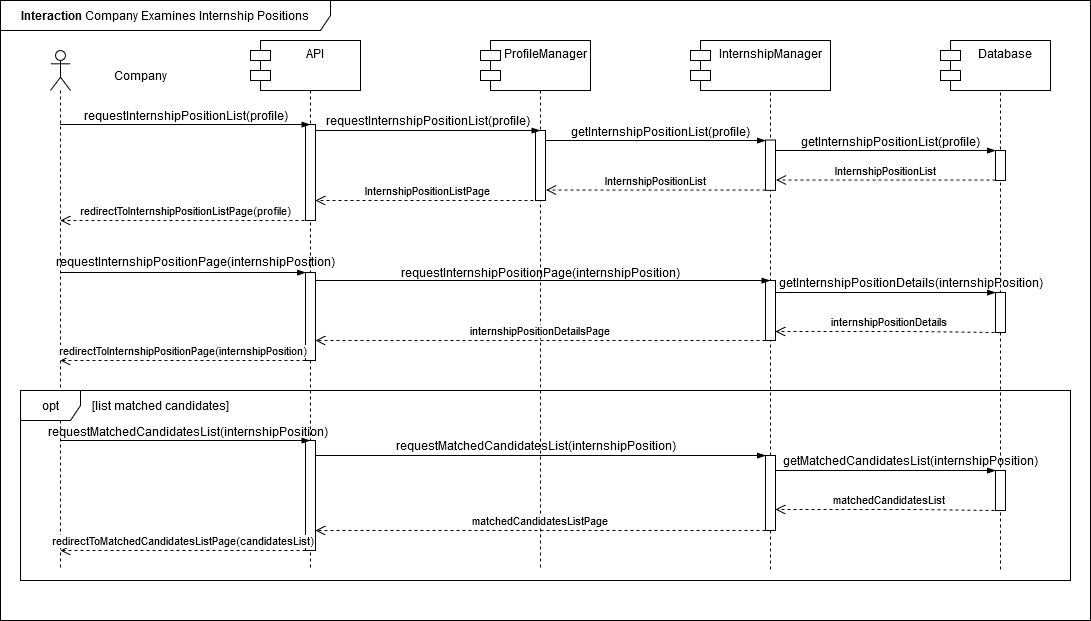
\includegraphics[width=1\textwidth]{DD/Images/Interactions/INT11_CompanyExaminesInternshipPosition.drawio.png}
            \label{fig:ComponentViewDiagram}
            \caption*{The interaction diagram shows the process of a company examining its internship positions within S\&C. The process begins when the user requests to view their internship positions history. This request is handled by the \textbf{API}, which redirects the user to the internship positions list page. The \textbf{API} communicates with the \textbf{ProfileManager} to retrieve the user’s profile-related data and then queries the \textbf{InternshipManager} for a list of the company’s internship positions.
            The \textbf{InternshipManager} consults the \textbf{Database} to gather the details of all internship positions associated with the user. 
            Once the information is retrieved, it is sent back to the \textbf{API}, which displays the internship positions list to the user on the internship positions list page.
            If the user selects a specific internship position for a detailed examination, the \textbf{API} processes this request by communicating with the \textbf{InternshipManager}. The \textbf{InternshipManager} retrieves the details of the selected internship position from the Database and sends them back to the \textbf{API}. Finally, the \textbf{API} redirects the user to a detailed view of the selected internship position, where they can review all relevant information.
            The company has also the option to examine the list of candidates and review their profiles. When requesting the list of candidates for a specific internship, the \textbf{API} communicates with the \textbf{InternshipManager}, which consults the \textbf{Database} to gather the information about each candidate. The data is sent back to the \textbf{InternshipManager}, which, through the \textbf{API}, redirects the company to the dedicated page displaying the list of matched candidates.
            }
    \end{figure}

    % -- INT12 --
    \newpage
    \item \textbf{Company Examines Internships}
    \begin{figure}[h!]
            \centering  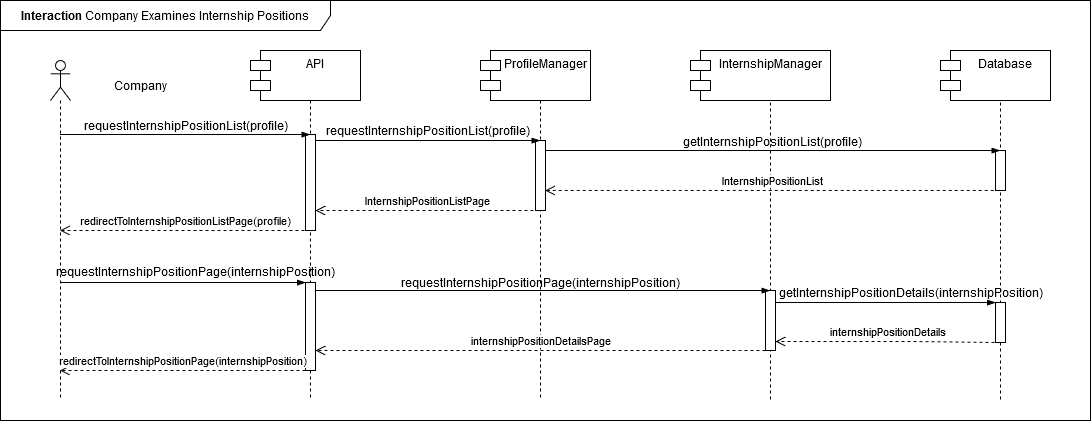
\includegraphics[width=1\textwidth]{DD/Images/Interactions/INT12_CompanyExaminesInternships.drawio.png}
            \label{fig:ComponentViewDiagram}
            \caption*{The interaction diagram shows the process of a company examining its internship within S\&C. The process begins when the user requests to view their internships history. This request is handled by the \textbf{API}, which redirects the user to the internship list page. The \textbf{API} communicates with the \textbf{ProfileManager} to retrieve the user’s profile-related data and then queries the \textbf{InternshipManager} for a list of the company’s internship.
            The \textbf{InternshipManager} consults the \textbf{Database} to gather the details of all internship associated with the user. 
            Once the information is retrieved, it is sent back to the \textbf{API}, which displays the internship list to the user on the internship list page.
            If the user selects a specific internship for a detailed examination, the \textbf{API} processes this request by communicating with the \textbf{InternshipManager}. The \textbf{InternshipManager} retrieves the details of the selected internship from the Database and sends them back to the \textbf{API}. Finally, the \textbf{API} redirects the user to a detailed view of the selected internship, where they can review all relevant information.
            }
    \end{figure}

    % -- INT13 --
    \newpage
    \item \textbf{Company Examines Applications}
    \begin{figure}[h!]
            \centering  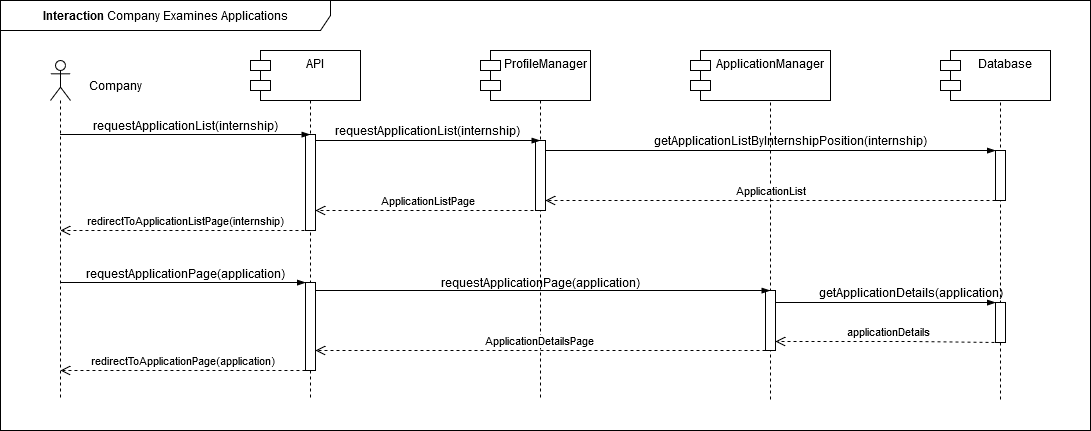
\includegraphics[width=1\textwidth]{DD/Images/Interactions/INT13_CompanyExaminesApplications.drawio.png}
            \label{fig:ComponentViewDiagram}
            \caption*{The interaction diagram shows the process of a company examining applications related to a specific internship within S\&C. The process begins when the user requests to view their applications history. This request is handled by the \textbf{API}, which redirects the user to the application list page. The \textbf{API} communicates with the \textbf{ProfileManager} to retrieve the internship data and then queries the \textbf{ApplicationManager} for a list of the students’ applications associated with the internship.
            The \textbf{ApplicationManager} consults the \textbf{Database} to gather details of all applications associated with the internship. 
            Once the information is retrieved, it is sent back to the \textbf{API}, which displays the applications list to the user on the applications list page.
            If the user selects a specific application for a detailed examination, the \textbf{API} processes this request by communicating with the \textbf{ApplicationManager}. The \textbf{ApplicationManager} retrieves the details of the selected application from the \textbf{Database} and sends them back to the \textbf{API}. Finally, the \textbf{API} redirects the user to a detailed view of the selected application, where they can review all relevant information.
            }
    \end{figure}

    % -- INT14 --
    \newpage
    \item \textbf{Application Acceptance or Rejection}
    \begin{figure}[h!]
            \centering  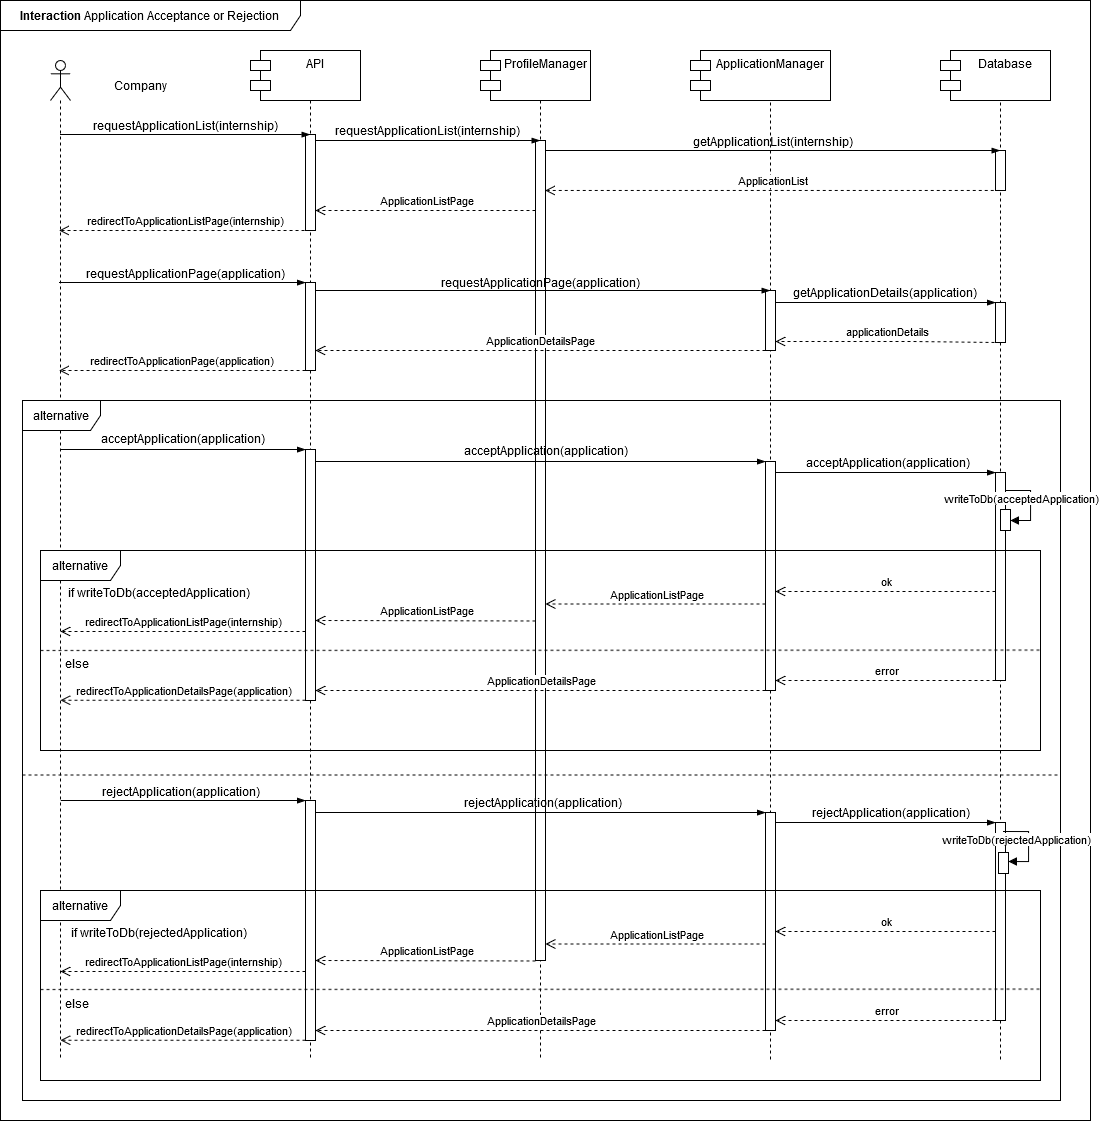
\includegraphics[width=1\textwidth]{DD/Images/Interactions/INT14_ApplicationAcceptanceOrRejection.drawio.png}
            \label{fig:ComponentViewDiagram}
    \end{figure}

    The interaction diagram shows the process of a company examining applications related to a specific internship and deciding to accept or reject a specific application within S\&C. The process begins when the user requests to view their applications history. This request is handled by the \textbf{API}, which redirects the user to the application list page. The \textbf{API} communicates with the \textbf{ProfileManager} to retrieve the internship data and then queries the \textbf{ApplicationManager} for a list of the students’ applications associated with the internship.
    The \textbf{ApplicationManager} consults the \textbf{Database} to gather details of all applications associated with the internship. 
    Once the information is retrieved, it is sent back to the \textbf{API}, which displays the applications list to the user on the applications list page.
    If the user selects a specific application for a detailed examination, the \textbf{API} processes this request by communicating with the \textbf{ApplicationManager}. The \textbf{ApplicationManager} retrieves the details of the selected application from the \textbf{Database} and sends them back to the \textbf{API}. 
    \\Finally, the \textbf{API} redirects the user to a detailed view of the selected application, where they can review all relevant information.
    At this point the company can choose to accept or reject the application by sending this decision to the \textbf{ApplicationManager} through the \textbf{API}. The \textbf{ApplicationManager} stores this new information into the \textbf{Database}. If the operation is successful, the \textbf{Database} sends a \textit{success message}, which allows first the \textbf{ApplicationManager} and then the \textbf{ProfileManager} to redirect the company back to the application list page through the \textbf{API}. 
    If there is any error during the write operation in the \textbf{Database}, the company is redirected to the application details page to address the issue.
    
    % -- INT15 --
    \newpage
    \item \textbf{Further Assessment for Application}
    \begin{figure}[h!]
            \centering  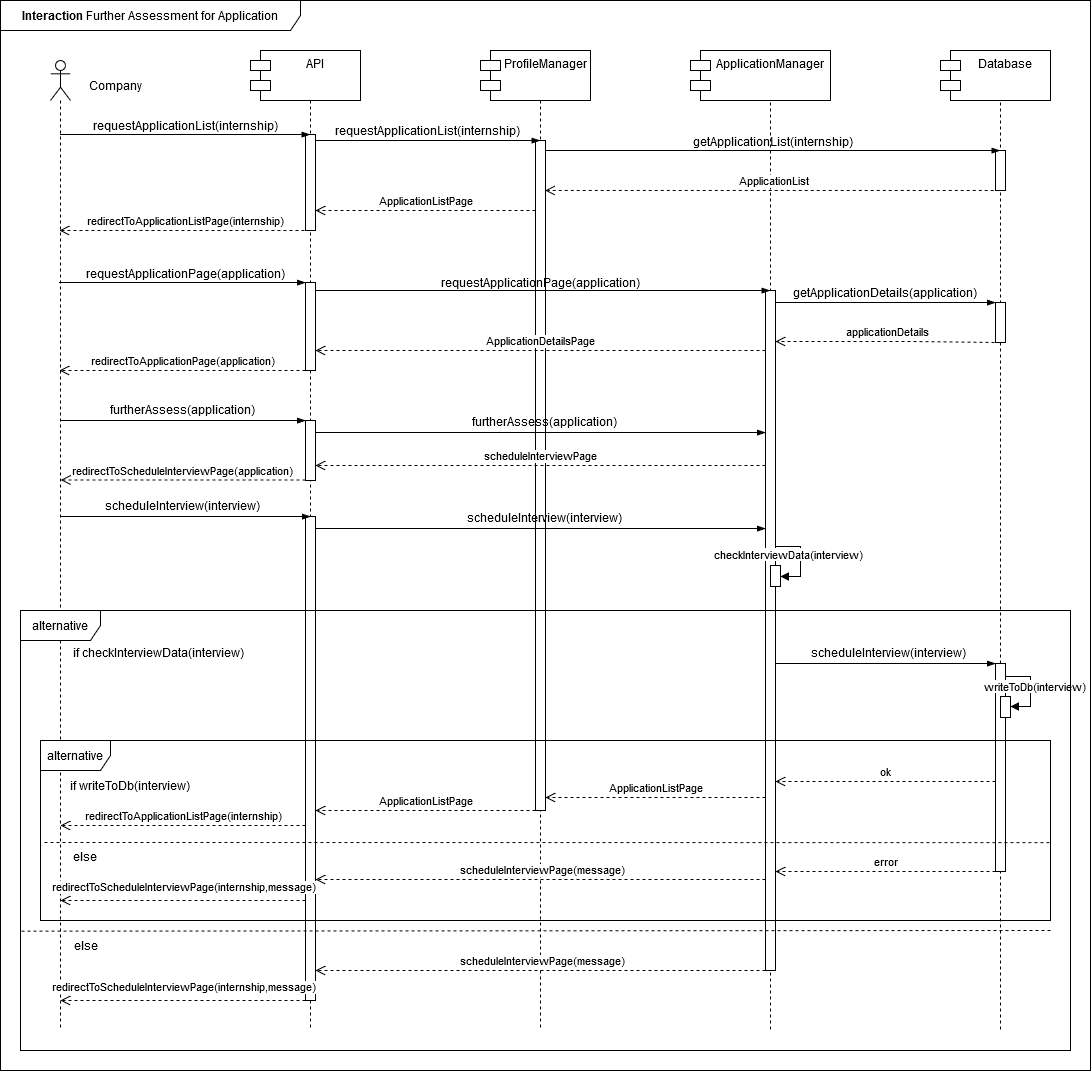
\includegraphics[width=1\textwidth]{DD/Images/Interactions/INT15_FurtherAssessmentForApplication.drawio.png}
            \label{fig:ComponentViewDiagram}
    \end{figure}

    The interaction diagram shows the process of a company examining applications related to a specific internship and deciding to have the candidate further evaluated within S\&C. The process begins when the user requests to view their applications history. This request is handled by the \textbf{API}, which redirects the user to the application list page. The \textbf{API} communicates with the \textbf{ProfileManager} to retrieve the internship data and then queries the \textbf{ApplicationManager} for a list of the students’ applications associated with the internship.
    The \textbf{ApplicationManager} consults the \textbf{Database} to gather details of all applications associated with the internship. 
    Once the information is retrieved, it is sent back to the \textbf{API}, which displays the applications list to the user on the applications list page.
    If the user selects a specific application for a detailed examination, the \textbf{API} processes this request by communicating with the \textbf{ApplicationManager}. The \textbf{ApplicationManager} retrieves the details of the selected application from the \textbf{Database} and sends them back to the \textbf{API}. 
    Finally, the \textbf{API} redirects the user to a detailed view of the selected application, where they can review all relevant information.
    At this point the company can decide to schedule an interview for a specific application by informing the \textbf{ApplicationManager} through the \textbf{API}, which redirects the user to the page where they can fill in all the required information to schedule the interview. This data is first sent to the \textbf{API} and then to the \textbf{ApplicationManager} for validation. If the check is successful, this information is stored in the \textbf{Database}. 
    If the operation is successful, the \textbf{Database} sends a \textit{success message}, which allows first the \textbf{ApplicationManager} and then the \textbf{ProfileManager} to redirect the company back to the application list page through the \textbf{API}. 
    If there is any error during the write operation in the \textbf{Database}, the company is redirected to the schedule interview page to address the issue.

    % -- INT16 --
    \newpage
    \item \textbf{Feedback from User}
    \begin{figure}[h!]
            \centering  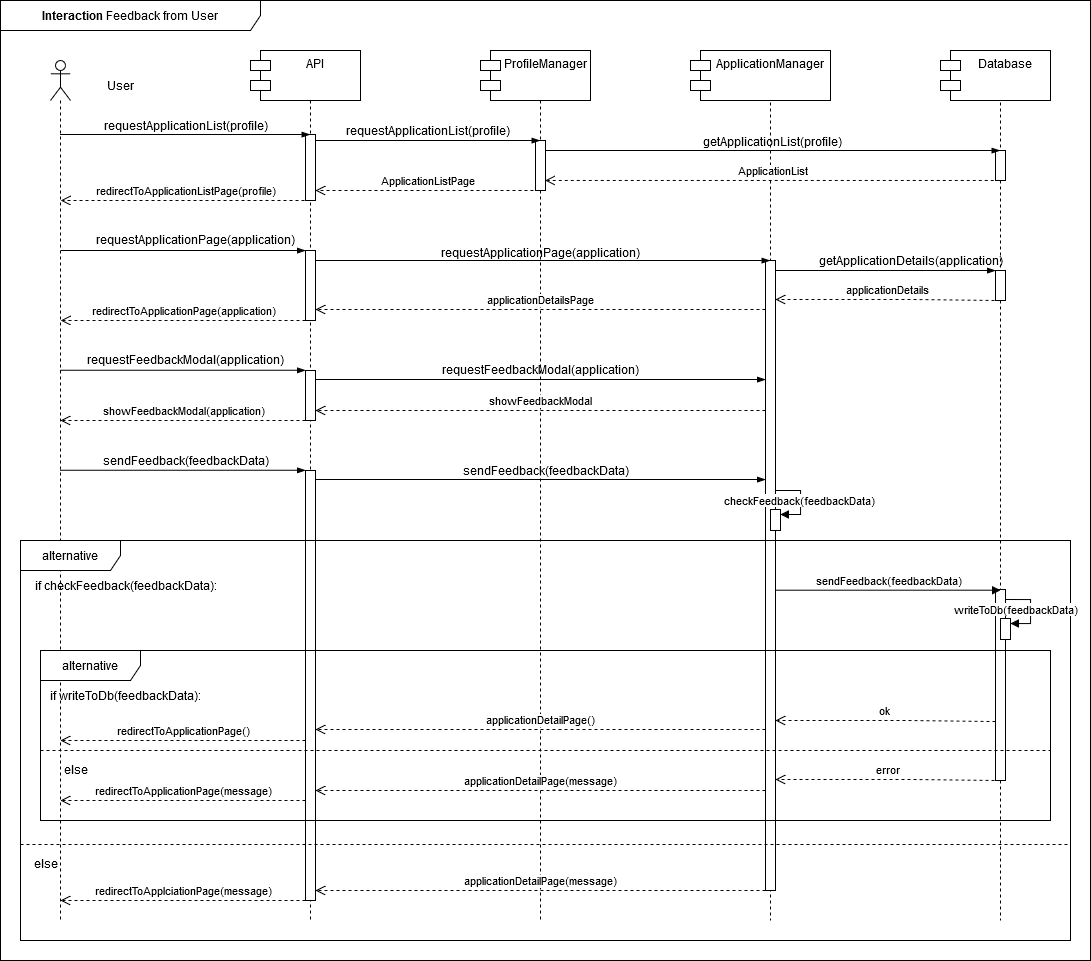
\includegraphics[width=1\textwidth]{DD/Images/Interactions/INT16_ FeedbackFromUser.drawio.png}
            \label{fig:ComponentViewDiagram}
    \end{figure}
            
    The interaction diagram shows the process of a user examining applications related to a specific internship and deciding to send a feedback within S\&C. The process begins when the user requests to view their applications history. This request is handled by the \textbf{API}, which redirects the user to the application list page. The \textbf{API} communicates with the \textbf{ProfileManager} to retrieve the internship data and then queries the \textbf{ApplicationManager} for a list of the students’ applications associated with the internship.
    The \textbf{ApplicationManager} consults the \textbf{Database} to gather details of all applications associated with the internship. 
    Once the information is retrieved, it is sent back to the \textbf{API}, which displays the applications list to the user on the applications list page.
    If the user selects a specific application for a detailed examination, the \textbf{API} processes this request by communicating with the \textbf{ApplicationManager}. The \textbf{ApplicationManager} retrieves the details of the selected application from the \textbf{Database} and sends them back to the \textbf{API}. 
    Finally, the \textbf{API} redirects the user to a detailed view of the selected application, where they can review all relevant information.
    At this point the user can decide to create a feedback for a specific application by informing the \textbf{ApplicationManager} through the \textbf{API}, which redirects the user to the page where they can fill in all the required information. This data is first sent to the \textbf{API} and then to the \textbf{ApplicationManager} for validation. If the check is successful, this information is stored in the \textbf{Database}. 
    If the operation is successful, the \textbf{Database} sends a \textit{success message}, which allows first the \textbf{ApplicationManager} and then the \textbf{ProfileManager} to redirect the user back to the application page through the \textbf{API}. 
    If there is any error during the write operation in the \textbf{Database}, the user is redirected to the application page with a message to address the issue.
    
    % -- INT17 --
    \newpage
    \item \textbf{Communication between Users}
    \begin{figure}[h!]
            \centering  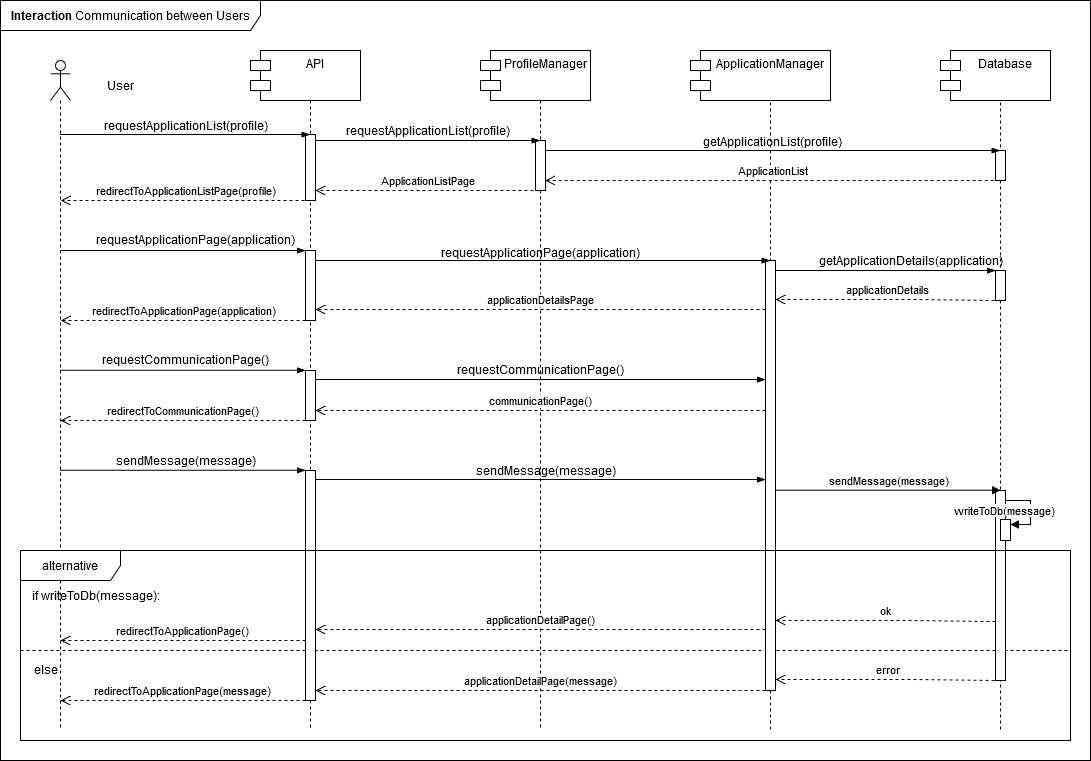
\includegraphics[width=1\textwidth]{DD/Images/Interactions/INT17_ CommunicationBetweenUsers.drawio.png}
            \label{fig:ComponentViewDiagram}
            \caption{
            The interaction diagram shows the process of a user examining applications related to a specific internship and deciding to send a message within S\&C. The process begins when the user requests to view their applications history. This request is handled by the \textbf{API}, which redirects the user to the application list page. The \textbf{API} communicates with the \textbf{ProfileManager} to retrieve the internship data and then queries the \textbf{ApplicationManager} for a list of the students’ applications associated with the internship.
            The \textbf{ApplicationManager} consults the \textbf{Database} to gather details of all applications associated with the internship. 
            Once the information is retrieved, it is sent back to the \textbf{API}, which displays the applications list to the user on the applications list page.
            If the user selects a specific application for a detailed examination, the \textbf{API} processes this request by communicating with the \textbf{ApplicationManager}. The \textbf{ApplicationManager} retrieves the details of the selected application from the \textbf{Database} and sends them back to the \textbf{API}. 
            Finally, the \textbf{API} redirects the user to a detailed view of the selected application, where they can review all relevant information.
            At this point the user can decide to create a message for a specific application by informing the \textbf{ApplicationManager} through the \textbf{API}, which redirects the user to the page where they can write the message. This data is first sent to the \textbf{API}, then to the \textbf{ApplicationManager} and finally is stored in the \textbf{Database}. 
            If the operation is successful, the \textbf{Database} sends a \textit{success message}, which allows first the \textbf{ApplicationManager} and then the \textbf{ProfileManager} to redirect    the user back to the application page through the \textbf{API}. 
            If there is any error during the write operation in the \textbf{Database}, the user is redirected to the application page with a message to address the issue.
            }
    \end{figure}
    
    
    % -- INT18 --
    \newpage
    \item \textbf{University Registration}
    \begin{figure}[h!]
            \centering  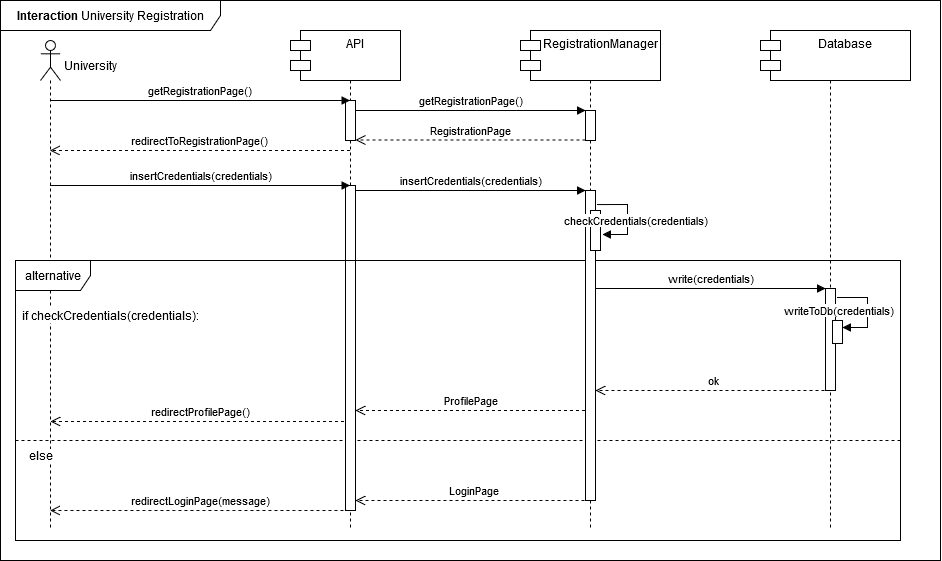
\includegraphics[width=1\textwidth]{DD/Images/Interactions/INT18_UniversityRegistration.drawio.png}
            \label{fig:ComponentViewDiagram}
            \caption*{The interaction diagram describes the process of university registration within the S\&C. The process begins when a university initiates a request to access the registration page. The \textbf{API} handles this request and redirects the university to the appropriate page for inputting registration details. Once the university provides its credentials, the \textbf{API} forwards the submitted information to the \textbf{RegistrationManager} that validates them, checking their correctness and ensuring they meet the necessary requirements. 
            If the validation is successful, the \textbf{RegistrationManager} stores the new credentials by writing them to the \textbf{Database}. After confirmation of successful storage, the \textbf{API} redirects the university to their newly created profile page. If the credentials fail validation due to errors or missing information, the \textbf{RegistrationManager} notifies the \textbf{API}. In this case, the \textbf{API} redirects the university back to the login page with an appropriate error message.
            }
    \end{figure}

    % -- INT19 --
    \newpage
    \item \textbf{University Monitors Internships}
    \begin{figure}[h!]
            \centering  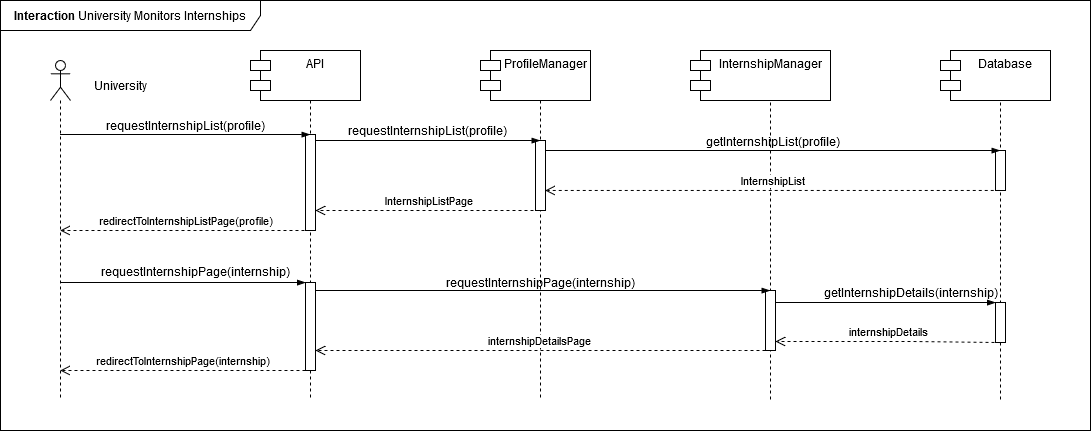
\includegraphics[width=1\textwidth]{DD/Images/Interactions/INT19_UniversityMonitorsInternships.drawio.png}
            \label{fig:ComponentViewDiagram}
            \caption*{The interaction diagram shows the process of a university examining internships of its students within S\&C. The process begins when the user requests to view their internships history. This request is handled by the \textbf{API}, which redirects the user to the internship list page. The \textbf{API} communicates with the \textbf{ProfileManager} to retrieve the user’s profile-related data and then queries the \textbf{InternshipManager} for a list of the internships of its students.
            The \textbf{InternshipManager} consults the \textbf{Database} to gather the details of all internship associated with the user. 
            Once the information is retrieved, it is sent back to the \textbf{API}, which displays the internship list to the user on the internship list page.
            If the user selects a specific internship for a detailed examination, the \textbf{API} processes this request by communicating with the \textbf{InternshipManager}. The \textbf{InternshipManager} retrieves the details of the selected internship from the Database and sends them back to the \textbf{API}. Finally, the \textbf{API} redirects the user to a detailed view of the selected internship, where they can review all relevant information.
            }
    \end{figure}
    
\end{enumerate}
\newpage
\subsection{Component Interfaces}
% To do 
\newpage
\subsection{Selected Architectural Styles and Patterns}
\subsubsection{3-Tier Architecture}
As already mentioned in the overview above, the decision to go for the 3-tier architecture is based on the belief that this type of architecture is well suited to the kind of application that it is going to be developed.
The first immediate benefit comes from the modularization which is the key feature of this type of architecture and from which indeed its name derives. The 3 independent layers are: 
\begin{itemize}
    \item \textbf{Presentation layer}: this corresponds to the front-end which is composed by the web pages and web interfaces with which the users interact.
    \item \textbf{Application layer}: this corresponds to the back-end which is where the logic of the application resides. 
    \item \textbf{Data layer}: this corresponds to the database which is the place where data are stored permanently.
\end{itemize}
The choice of implementing a three-tier architecture has several advantages.
\begin{itemize}
    \item The various tiers can be developed simultaneously and independently by different people or teams of people making the development phase faster
    \item The division in three tiers makes the separation of different functions more clear and makes the code easier to be understood and maintained
    \item The separation in three allows each layer to be scaled independently from the others, thus enhancing the overall scalability of the web application
\end{itemize}
To facilitate the communication between the presentation  and the application layers we decided to adopt the use of REST APIs. This choice brings many advantages:
\begin{itemize}
    \item \textbf{Decoupling}: it allows the developers to separate the scope and the concerns of the modules in three different layers, making the maintenance of the web application and the deployment of new features easier.
    \item \textbf{Easier future integration with third party services}: if for any reason in the future it will be necessary to add third party services they could be  effortlessly integrated into the system. 
    \item \textbf{Standard formats of communication}: REST APIs use standard HTTP methods and the JSON format to communicate which are the common standard for the world wide web.
    \item \textbf{Scalability}: each tier can be scaled independently from the others (up to a certain point of course).
\end{itemize}
\subsection{Other Design Decisions}

\subsubsection{Standard Compliance}
S\&C should be GDPR compliant, therefore when deployed into production must use cloud providers that keep the European citizen's data in the EU. Moreover, it will use encryption libraries (such as Flask BCrypt) to securely store sensitive information. 

\subsubsection{Security}
The code infrastructure will use a secure-by-design approach, creating secure code and test it really extensively in order to discover bugs and vulnerabilities before the deployment. Some libraries that are going to be used towards the goal of making the web application secure are Flask Cors, JWT, BCrypt on the back-end and custom validation code on the front-end. More information on the testing plan will be discussed in section 5 of this document.

\subsubsection{Reliability}
S\&C must be reliable and therefore enforce data consistency.For this reason we thought that a SQL database is a good choice. For prototyping SQLite is definitely the best choice, when going to production solid choices are PostgreSQL and MySQL.

\subsubsection{Availability}
S\&C must be available as much as possible. Therefore, it is important that the code written allows the server to be up and running smoothly.

\subsubsection{Maintainability}
S\&C code base should be easily maintainable. In order to ensure that, first of all, no legacy code will be allowed. Legacy code slow the web app down: all the lies of code in the project must have a purpose. Modular programming is strongly recommended. Modules enhance readability of the code, allow for decoupling of components and, in general, help when in case of debugging. GitHub will be used as a versioning control software to keep track of the changes of the code and their authors. Comments are also strongly recommended: commenting functions, APIs and more generally anything that it is not immediately clear is a good programming practice.